\documentclass[14pt]{beamer}
\usetheme{Warsaw}
\usecolortheme{beaver}
\usefonttheme{professionalfonts}

\input{../../preamble}
\usepackage{amscd,amsmath,amssymb,amsthm,graphicx}
\usepackage[mathscr]{eucal}
\usepackage{paralist}
\usepackage{tabto}
\usepackage[normalem]{ulem}

% % % % % % % % % %
\title[Cal I S2015]{MATH 2554 (Calculus I)}
\subtitle{}
\author[Wheeler]{Dr. Ashley K. Wheeler}
\institute{University of Arkansas}
\date{\today}
\logo{}

% % %
\begin{document}
\maketitle

% % %
\begin{frame}
\frametitle{Table of Contents}
\tableofcontents
\end{frame}

% % % % % % % % % % Mon 26 Jan 2015

% % %
\begin{frame}
\section[Week 3]{Week 3: 26-30 January}
\frametitle{Monday 26 January (Week 3)}
\footnotesize
\begin{itemize}
\item MAA quiz results 
	\begin{itemize}
	\footnotesize
	\item posted on MLP soon
	\item originally out of 25 
	\item grading: your raw score taken out of 15, then scaled to out of 10
	\item If your raw score was 15/25 or higher then you got 10/10. 
	\end{itemize}
\item Quizzes: Hold on to your old quizzes, for studying, computing your grade, etc.
\item Thurs 29 Jan Quiz 3 
\item 3rd WebHW is live.
\item EXAM \#1: Friday 6 February 
	\begin{itemize}
	\footnotesize
	\item in class
	\item covers up to and including $\oint 3.1$
	\end{itemize}
\end{itemize}
\end{frame}

% % %
\subsection[2.5 Limits at Infinity, cont.]{$\oint$ 2.5 Limits at Infinity, cont.}
% % %

% % %
\begin{frame}
\frametitle{(recall, from $\oint 2.5$ Limits at Infinity)}
\footnotesize
{\bf Rational Functions:}  Suppose $f(x)=\dfrac{p(x)}{q(x)}$ is a rational function.

\begin{itemize}
\item[{\bf 1.}] If $\deg(p)<\deg(q)$, i.e., \alert{the numerator has the smaller degree}, then 
\[\lim_{x\to\pm\infty}f(x)=0\] 
(also, $y=0$ is a horizontal asymptote of $f$).

\vspace{2pc}
\item[{\bf 2.}] If $\deg(p)=\deg(q)$, i.e., \alert{numerator and denominator have the same degree}, then 
\[\lim_{x\to\pm\infty}f(x)=\dfrac{\text{lc}(p)}{\text{lc}(q)},\] 
and $y=\dfrac{\text{lc}(p)}{\text{lc}(q)}$ is a horizontal asymptote of $f$.
\end{itemize}
\end{frame}

% % %
\begin{frame}
\frametitle{(recall, from $\oint 2.5$)}
\begin{itemize}
\small
\item[{\bf 3.}] If $\deg(p)>\deg(q)$, \alert{(numerator has the bigger degree)} then 
\[\lim_{x\to\pm\infty}f(x)=\infty\quad\text{or}\quad -\infty\] 
and $f$ has no horizontal asymptote.

\vspace{2pc}
\item[{\bf 4.}] Assuming that $f(x)$ is in \alert{reduced form} ($p$ and $q$ share no common factors), vertical asymptotes occur at the zeroes of $q$.  

\vspace{1pc}
(This is why it is a good idea to check for factoring and cancelling first!)
\end{itemize}
\end{frame}

% % %
\begin{frame}
\frametitle{(recall, from $\oint 2.5$)}
\small
{\bf Pneumonic for limits at infinity for rational functions:}
\begin{block}
{BOB0}
\alert{B}igger \alert{O}n \alert{B}ottom \alert{0}
\end{block}
\begin{block}
{BOTN}
\alert{B}igger \alert{O}n \alert{T}op \alert{N}either
\end{block}
\begin{block}
{BETC (Betsy)}
\alert{B}ottom \alert{E}quals \alert{T}op \alert{C}oefficient
\end{block}
\end{frame}

% % %
\begin{frame}
\frametitle{(recall, from $\oint 2.5$)}
\small
{\bf Algebraic and Transcendental Functions:}

Determine the end behavior of the following functions.
\begin{itemize}
\item $f(x) = \dfrac{4x^3}{2x^3+\sqrt{9x^6+15x^4}}$ (radical signs appear)

\vspace{1pc}
\item $g(x)=\cos x$ (trig)

\vspace{1pc}
\item $h(x)=e^x$ (exponential)
\end{itemize}
\end{frame}

% % %
\begin{frame}
\frametitle{HW from Section 2.5}
Do problems 9--10, 13--35 odds, 39, 43, 45, 53 (pp.\ 92--93 in textbook)
\end{frame}

% % %
\subsection[2.6 Continuity]{$\oint$ 2.6 Continuity}
% % %

% % %
\begin{frame}
\frametitle{$\oint$ 2.6 Continuity}
\small
{\bf Informal Def.:} A function $f$ is continuous at $x=a$ means near $x=a$ the graph can be drawn without lifting a pencil.  In other words, no holes, breaks, asymptotes, etc.

\vspace{1pc}
{\bf Formal Def.:} A function $f$ is continuous at $a$ means
\[\lim_{x \to a} f(x)=f(a).\]  
If $f$ is not continuous at $a$, then $a$ is a point of discontinuity.
\end{frame}

% % %
\begin{frame}
\frametitle{Continuity Checklist}
\small
In order to claim something is continuous, you must verify all three:

\begin{itemize}
\item[1.] \alert{$f(a)$ is defined} (i.e., $a$ is in the domain of $f$ -- no holes, asymptotes).

\vspace{0.5pc}
\item[2.] \alert{$\displaystyle\lim_{x \to a} f(x)$ exists.}  You must check both sides and make sure they equal the same number.

\vspace{0.5pc}
\item[3.] \alert{$\displaystyle\lim_{x \to a} f(x) = f(a)$} (i.e., the value of $f$ equals the limit of $f$ at $a$).  What is an example of a function that satisfies this condition?
\end{itemize}
\end{frame}

% % %
\begin{frame}
\small
Where are the points of discontinuity of the function below?  Which aspects of the checklist fail?
\begin{columns}[T]
	\begin{column}{.45\textwidth}
		\begin{block}
		\centering{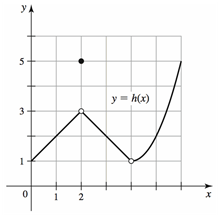
\includegraphics[scale=0.75]{Ch2Sect2_Exer7}}
		\end{block}
	\end{column}
	\begin{column}{.45\textwidth}
		\begin{block}
		{Checklist:}
			\begin{itemize}
			\item[1.] function is defined
			\item[2.] the two-sided limit exists
			\item[3.] 2.\;=\;1.
			\end{itemize}
		\end{block}
	\end{column}
\end{columns}
\end{frame}

% % %
\begin{frame}
\frametitle{}
\small
{\bf Continuity Rules:}  If $f$ and $g$ are continuous at $a$, then the following functions are also continuous at $a$.  Assume $c$ is a constant and $n>0$ is an integer.

\begin{itemize}
\item[1.] $f+g$
\item[2.] $f-g$
\item[3.] $cf$
\item[4.] $fg$
\item[5.] $\frac{f}{g}$, provided $g(a)\ne 0$
\item[6.] $[f(x)]^n$
\end{itemize}
\end{frame}

% % %
\begin{frame}
\frametitle{}
{\bf From the rules above, we can deduce:}

\begin{itemize}
\item[1.] Polynomials are continuous for all $x=a$.
\item[2.] Rational functions are continuous at all $x=a$ except for the points where the denominator is zero.  
\item[3.] If $g$ is continuous at $a$ and $f$ is continuous at $g(a)$, then the composite function $f \circ g$ is continuous at $a$.
\end{itemize}
\end{frame}

% % % % % % % % % % Wed 28 Jan 2015

% % %
\begin{frame}
\frametitle{Wednesday 28 January (Week 3)}
\footnotesize
\begin{itemize}
\item Quizzes: 
	\begin{itemize}
	\footnotesize
	\item MAA quiz results ...
	\item Double check the solutions for Quiz 1 -- corrections are posted.
	\item Hold on to your old quizzes, for studying, computing your grade, etc.
	\item See me (OH) if you have questions about quizzes or computing your grade.
	\end{itemize}
\item Thurs 29 Jan Quiz 3 
\item EXAM \#1: Friday 6 February 
	\begin{itemize}
	\footnotesize
	\item in class
	\item covers up to and including $\oint 3.1$
	\end{itemize}
\item See the course schedule: Monday is $\oint 3.1$ but if possible we will start it on Friday.  Wednesday is review for the exam.	
\end{itemize}
\end{frame}

% % %
\begin{frame}
\frametitle{($\oint 2.6$)}
\small
{\bf Continuity on an Interval:} Consider the cases where $f$ is not defined past a certain point.  (e.g., $\ln x$)

\vspace{1pc}
A function $f$ is continuous from the left (or left-continuous) at $a$ if
\[\lim_{x \to a^-} f(x)=f(a).\]

\vspace{0.5pc}
A function $f$ is continuous from the right (or right-continuous) at $a$ if
\[\lim_{x \to a^+} f(x)=f(a).\]
\end{frame}

% % %
\begin{frame}
\frametitle{($\oint 2.6$)}
A function $f$ is \alert{continuous on an interval $I$} means it is continuous at all points of $I$.  

\vspace{1.5pc}
Notation: Intervals are usually written 
\[\left[a,b\right],\;\left(a,b\right],\;\left[a,b\right),\text{ or }\left(a,b\right).\]

\vspace{1pc}
When $I$ contains its endpoints, ``continuity on $I$" means continuous from the right or left at the endpoints.
\end{frame}

% % %
\begin{frame}
\frametitle{Example}
Let $f(x)=
\begin{cases}
x^3+4x+1 & \text{if}\ x \leq 0 \\
2x^3 & \text{if}\ x>0.
\end{cases}$

\vspace{1pc}
\begin{itemize}
\item[1.] Use the continuity checklist to show that $f$ is not continuous at 0.

\vspace{0.5pc}
\item[2.] Is $f$ continuous from the left or right at 0?

\vspace{0.5pc}
\item[3.] State the interval(s) of continuity.
\end{itemize}
\end{frame}

% % %
\begin{frame}
\frametitle{Continuity of Functions with Roots}
\small
(assuming $m$ and $n$ are positive integers and $n/m$ is in lowest terms)

\vspace{0.5pc}
\begin{itemize}
\small
\item If $m$ is odd, then $[f(x)]^{n/m}$ is continuous at all points at which $f$ is continuous.

\vspace{0.5pc}
\item If $m$ is even, then $[f(x)]^{n/m}$ is continuous at all points $a$ at which $f$ is continuous \alert{and $f(a)\geq 0$}.
\end{itemize}
\begin{que}  Where is $f(x)=\sqrt[4]{4-x^2}$ continuous?\end{que}
\end{frame}

% % %
\begin{frame}
\frametitle{Continuity of Transcendental Functions}
\footnotesize
{\bf Trig Functions:} The basic trig functions are all continuous at all points \alert{IN THEIR DOMAIN}.  Note there are points of discontinuity where the functions are not defined -- for example, $\tan x$ has asymptotes at multiples of $\pi$.

\vspace{1pc}
{\bf Exponential Functions:}  The exponential functions $b^x$ and $e^x$ are continuous on all points of their domains.

\vspace{1pc}
{\bf Inverse Functions:}  If a continuous function $f$ has an inverse on an interval $I$ (meaning if $x\in I$ then $f^{-1}(y)$ passes the vertical line test), then its inverse $f^{-1}$ is continuous on the interval $J$, which is defined as all the numbers $f(x)$, given $x$ is in $I$.
\end{frame}

% % %
\begin{frame}
\frametitle{Intermediate Value Theorem}
\small
\begin{thm}[Intermediate Value Theorem] Suppose \alert{$f$ is continuous on the interval $[a,b]$} and $L$ is a number satisfying
\[\alert{f(a)<L<f(b)\quad\text{or}\quad f(b)<L<f(a)}.\]  
Then there is at least one number $c\in (a,b)$, i.e., $a<c<b$, satisfying 
\[f(c)=L.\] \end{thm}

{\bf Example:}  Let $f(x)=-x^5-4x^2+2\sqrt{x}+5.$  Use IVT to show that $f(x)=0$ has a solution in the interval $(0,3)$.
\end{frame}

% % %
\begin{frame}
\frametitle{HW from Section 2.6}
Do problems 9--23 odds, 29--37 odds, 45, 49, 51, 53 (pp.\ 103--105 in textbook)
\end{frame}

% % % % % % % % % % Fri 30 Jan 2015

% % %
\begin{frame}
\frametitle{Friday 30 January (Week 3)}
\begin{itemize}
\item EXAM \#1: Friday 6 February 
	\begin{itemize}
	\footnotesize
	\item in class
	\item covers up to and including $\oint 3.1$
	\end{itemize}
\item See the course schedule: Monday is $\oint 3.1$ but if possible we will start it today.  Wednesday is review for the exam.	
\end{itemize}
\end{frame}

% % %
\subsection[2.7 Precise Definitions of Limits]{$\oint$ 2.7 Precise Definitions of Limits}
% % %

% % %
\begin{frame}
\frametitle{$\oint$ 2.7 Precise Definitions of Limits}
\small
Assume that $f(x)$ exists for all $x$ in some open interval (open means: neither of the endpoints not included) containing $a$, except possibly at $a$.  

\vspace{1pc}
\alert{``The limit of $f(x)$ as $x$ approaches $a$ is $L$"}, i.e.,
\[\lim_{x \to a}f(x)=L,\]
means \alert{for any $\epsilon > 0$ there exists $\delta > 0$ such that} 
\[\alert{|f(x)-L|<\epsilon \quad \text{whenever} \quad 0<|x-a|<\delta.}\]
\end{frame}

% % %
\begin{frame}
\frametitle{Seeing $\epsilon$s and $\delta$s on a Graph}
\begin{columns}[T]
	\begin{column}{.5\textwidth}
		\begin{block}
		\centering{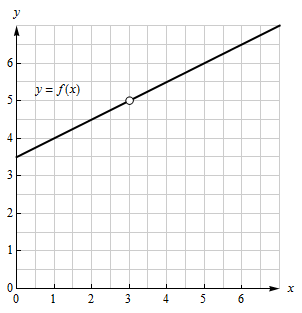
\includegraphics[scale=0.65]{Fig2_57}}
		\end{block}
	\end{column}
	\begin{column}{.5\textwidth}
		\begin{block}
		{Problem:} \footnotesize Using the graph, for each $\epsilon >0$, determine a value of $\delta>0$ to satisfy the statement 
		\begin{multline*}|f(x)-5|<\epsilon\quad\text{whenever} \\
			0<|x-3|<\delta.\end{multline*}  
		\vspace{-1pc}
		\begin{itemize}
		\item $\epsilon=1$ 
		\item $\epsilon=0.5$.
		\end{itemize}
		\end{block}
	\end{column}
\end{columns}
\end{frame} 

% % %
\begin{frame}
\frametitle{Seeing $\epsilon$s and $\delta$s on a Graph}
\small When $\epsilon=1$:

\vspace{-1pc}
\begin{columns}[T]
\begin{column}{.5\textwidth}
\begin{block}
\centering{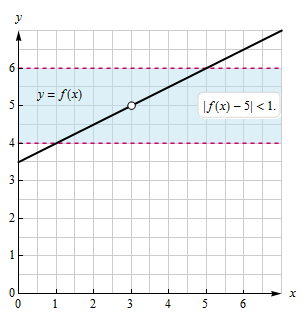
\includegraphics[scale=0.58]{Fig2_57a}}
\end{block}
\end{column}
\begin{column}{.5\textwidth}
\begin{block}
\centering{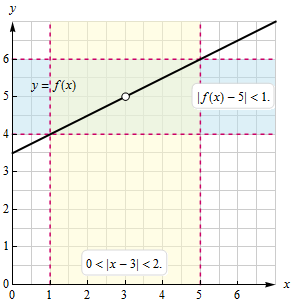
\includegraphics[scale=0.6]{Fig2_57b}}
\end{block}
\end{column}
\end{columns}
\vspace{-1pc}
\flushright $\dots\;\delta=2$
\end{frame}

% % %
\begin{frame}
\frametitle{Seeing $\epsilon$s and $\delta$s on a Graph}
\small When $\epsilon=0.5$:

\vspace{-1pc}
\begin{columns}[T]
\begin{column}{.5\textwidth}
\begin{block}
\centering{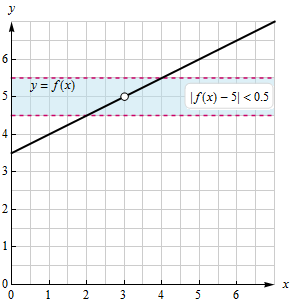
\includegraphics[scale=0.6]{Fig2_58}}
\end{block}
\end{column}
\begin{column}{.5\textwidth}
\begin{block}
\centering{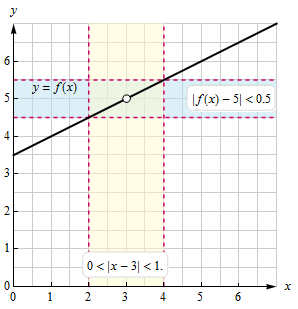
\includegraphics[scale=0.6]{Fig2_58a}}
\end{block}
\end{column}
\end{columns}
\flushright $\dots\;\delta=1$
\end{frame}

% % %
\begin{frame}
\frametitle{}
The $\epsilon$s and $\delta$s give a way to visualize computing the limit, and proving it exists.  As the $\epsilon$s get smaller and smaller, we want there to always be a $\delta$.  

\vspace{1pc}
In this example,
\[\lim_{x\to 3}f(x)=5.\]
\end{frame}

% % %
\begin{frame}
\begin{columns}[T]
	\begin{column}{.5\textwidth}
		\begin{block}
		\centering{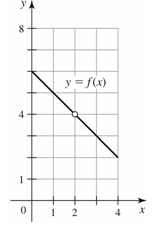
\includegraphics[scale=1.0]{Ch2Sect7_Exer10}}
		\end{block}
	\end{column}
	\begin{column}{.5\textwidth}
		\begin{block}
		{Exercise} \footnotesize Using the graph, for each $\epsilon>0$, determine a value of $\delta>0$ to satisfy the statement
		\begin{multline*}|f(x)-4|<\epsilon\quad\text{whenever} \\
			0<|x-2|<\delta.\end{multline*}  
		\vspace{-1pc}
		\begin{itemize}
		\item $\epsilon=1$ 
		\item $\epsilon=0.5$.
		\end{itemize}
		\end{block}
	\end{column}
\end{columns}
\end{frame} 

% % %
\begin{frame}
\frametitle{}
{\bf Exercise:}
Let $f(x)=x^2-4$.  For $\epsilon=1$, find a value for $\delta>0$ so that 
\[|f(x)-12|<\epsilon \quad \text{whenever}\quad 0<|x-4|<\delta.\]

\vspace{1pc}
In this example,  $\displaystyle\lim_{x \to 4}f(x)=12.$  
\end{frame}

% % %
\begin{frame}
\frametitle{Finding a Symmetric Interval}
\begin{que}When finding an interval $(a-\delta, a+\delta)$ around the point $a$, what happens if you compute two different $\delta$s?\end{que}  

\vspace{1pc}
{\bf Answer:}  To obtain a symmetric interval around $a$, use the smaller of the two $\delta$s as your distance around $a$.
\end{frame}

% % %
\begin{frame}
\begin{columns}[T]
	\begin{column}{.5\textwidth}
		\begin{block}
		\centering{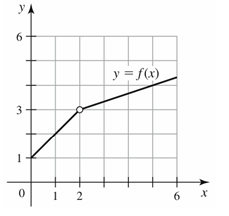
\includegraphics[scale=0.9]{Ch2Sect7_Exer15}}
		\end{block}
	\end{column}
	\begin{column}{.5\textwidth}
		\begin{block}
		{Exercise} \footnotesize The graph below shows $f(x)$ with 
		\[\lim_{x \to 2}f(x)=3.\] 
		For $\epsilon=1$, find the corresponding value of $\delta>0$ so that
		\begin{multline*}|f(x)-3|<\epsilon\quad\text{whenever} \\
			0<|x-2|<\delta.\end{multline*}  
		\end{block}
	\end{column}
\end{columns}
\end{frame}

% % %
\begin{frame}
\frametitle{HW from Section 2.7}
Do problems 1--7, 9--18 (pp.\ 115--116)
\end{frame}

% % %
\subsection[3.1 Introducing the Derivative]{$\oint$ 3.1 Introducing the Derivative}
% % %

% % %
\begin{frame}
\frametitle{$\oint$ 3.1 Introducing the Derivative}
\small
{\bf Recall from Ch 2:}  We said that the slope of the tangent line at a point is the limit of the slopes of the secant lines as the points get closer and closer.

\vspace{0.5pc}
%Let $P=(a,f(a))$ and $Q=(x,f(x))$.

\begin{itemize}
\item slope of secant line:  $\dfrac{f(x)-f(a)}{x-a}$\ (avg.\ rate of change) 

\vspace{0.5pc}
\item slope of tangent line:  $\displaystyle\lim_{x \to a} \frac{f(x)-f(a)}{x-a}$\ (instantaneous rate of change)
\end{itemize}
\end{frame}


% % %
\begin{frame}

Use the relationship between secant lines and tangent lines, specifically the slope of the tangent line, to find the equation of a line tangent to the curve $f(x)=x^2+2x+2$ at the point $P=(1,5)$.

\end{frame}

\begin{comment}
\begin{frame}

Instead of looking at the points approaching one another, we can also view this as the distance between the points approaching 0.  

\bigskip

For $P=(a,f(a))$, $Q=(a+h,f(a+h))$,

\bigskip

slope of secant line:  $\dfrac{f(a+h)-f(a)}{(a+h)-a}= \dfrac{f(a+h)-f(a)}{h}$\\

\bigskip

slope of tangent line:  $\displaystyle\lim_{h \to 0} \frac{f(a+h)-f(a)}{h}$

\end{frame}

\begin{frame}

Find the equation of a line tangent to the curve $f(x)=x^2+2x+2$ at the point $P=(2,10).$

\end{frame}

\begin{frame}

\frametitle{Def.\ of Derivative}

The slope of the tangent line for the function $f$ is a function of $x$, called the derivative of $f$.

\bigskip

The derivative of $f$ is the function 
$$f^{\prime}(x)=\lim_{h \to 0} \frac{f(x+h)-f(x)}{h}$$
provided the limit exists.  If $f^{\prime}(x)$ exists, we say $f$ is differentiable at $x$.  If $f$ is differentiable at every point of an open interval $I$, we say that $f$ is differentiable on $I$.

\end{frame}

\begin{frame}

Use the definition of the derivative to find the derivative of the function $f(x)=x^2+2x+2.$

\end{frame}

\begin{frame}

\frametitle{Alternate Notation}

A standard notation for change involves the Greek letter $\Delta$.  So
$$\frac{f(a+h)-f(a)}{h}=\frac{f(x+\Delta x)}{\Delta x}=\frac{\Delta y}{\Delta x}.$$

\bigskip

Additionally,
$$f^{\prime}(x)=\lim_{\Delta x \to 0} \frac{f(x+\Delta x)}{\Delta x}=\lim_{\Delta x \to 0} \frac{\Delta y}{\Delta x}=\frac{dy}{dx}.$$

\end{frame}

\begin{frame}

\frametitle{Other ways to write derivative}

The following are alternative ways of writing the derivative of the function $f$ at the point $x$:

$$\frac{dy}{dx}, \frac{df}{dx}, \frac{d}{dx}(f(x)), D_x (f(x)), y^{\prime}(x).$$

\bigskip

The following are ways to notate the derivative of $f$ evaluated at $x=a$:

$$f^{\prime}(a), y^{\prime}(a), \left. \frac{df}{dx} \right|_{x=a}, \left. \frac{dy}{dx} \right|_{x=a}$$

\end{frame}

\begin{frame}

\frametitle{Graphing the derivative}

The graph of the derivative is the graph of the collection of slopes of tangent lines of a graph.  If you just have a graph (without an equation for the graph), the best you can do is approximate the graph of the derivative.

\bigskip

Simple checklist:

\begin{itemize}

\item[1.] Note where $f^{\prime}(x)=0$.

\item[2.]  Note where $f^{\prime}(x)>0$.  (What does this look like?)

\item[3.]  Note where $f^{\prime}(x)<0$.  (What does this look like?)

\end{itemize}

\end{frame}

\begin{frame}

\frametitle{Differentiability and Continuity}

Key points about the relationship between differentiability and continuity:

\begin{itemize}

\item If $f$ is differentiable at $a$, then $f$ is continuous at $a$.

\item If $f$ is not continuous at $a$, then $f$ is not differentiable at $a$.

\item $f$ can be continuous at $a$, but not differentiable at $a$.

\end{itemize}

\end{frame}

\begin{frame}

\frametitle{When is a function not differentiable at a point?}

A function $f$ is \underline{not} differentiable at $a$ if at least one of the following conditions holds:

\begin{itemize}

\item[1.] $f$ is not continuous at $a$.

\item[2.] $f$ has a corner at $a$.  (Why does this make $f$ not differentiable?)

\item[3.] $f$ has a vertical tangent at $a$.  (Why does this make $f$ not differentiable?)

\end{itemize}

\end{frame}

\begin{frame}

\frametitle{HW from Section 3.1}  

Do problems 11--12, 19--20, 23--26, 31--33, 35--36, 39--43, 45, 49--52 (pp.\ 131--133 in textbook)

\bigskip

{\bf NOTE:}  You do not know any rules for differentiation yet (e.g., Power Rule, Chain Rule, etc.)  In this section, you are strictly using the definition of the derivative and the definition of slope of tangent lines we have derived.

\end{frame}

\end{comment}

\end{document}